This example is a tracking problem. 
Markers trajectories, ground reaction forces and moments were tracked. 
The goal was to estimate muscles activation during one gait cycle from the first heel strike to the end of the swing phase using a 3D one-leg model with 12 DoFs and 17 muscles. 
Residual torques were also added to compensate model weaknesses providing pure joint torque in addition to muscle-induced ones.\\

This tracking optimization consisted in the minimization between predicted $m_p$ and measured $m_m$ markers trajectories. 
During the stance phase, predicted forces $F_c$ at C contact point and computed moments 
were compared to measured ground reaction forces $F_m$ and moments $M_{m,O}$.
To predict muscle activity, the objective function consisted in finding the least squared muscle activations $a_{i}$. 
The objective functions are written as follow :\\


\begin{eqnarray}
\label{eq:ocp_q}
\mathcal{J} = \sum_{i=1}^{N_i}\Bigg(\underbrace{\omega_1(\|m_p - m_m\|^{2})}_{TRACK\_MARKERS}
\label{eq:ocp_forces}
\end{eqnarray}
\begin{eqnarray}
+ \underbrace{\omega_2(\|\sum_{c=1}^{N_c}F_c - F_m\|^{2})}_{TRACK\_FORCES}
\end{eqnarray}
\begin{eqnarray}
\label{eq:ocp_moments}
+ \underbrace{\omega_3(\|\sum_{c=1}^{N_c}OC\times F_c - M_{m,O}\|^{2})}_{TRACK\_MOMENTS}
\end{eqnarray}
\begin{eqnarray}
\label{eq:ocp_muscles}
+ \underbrace{\omega_4\int_0^T \sum_{i=1}^{N_i}~a_{i}^2~dt}_{MINIMIZE\_ ACTIVATION}\bigg)  
\end{eqnarray}

where $\omega_1$, $\omega_2$, $\omega_3$, $\omega_4$ are weighting factors, $T$ is the the duration, $N_i$ and $N_c$ are the number of time frames and contact points of the current phase. \\


The interaction between the ground and the foot was modelled using a 4-contact points model located at the heel and the forefoot (first, fifth metatarsi and hallux). 
The stance phase was divided in three to follow the natural rolling movement of the foot from heel strike to toe off: heel, flatfoot and forefoot contacts. 
A constraint of non-slipping (NON\_SLIPPING) and unilateral contact force (CONTACT\_FORCE) were added. 
It prevents the foot from slipping and penetrating the ground. 
The use of the IMPACT state transition allowed to represent the gain of contact(s) from a system without any contact (swing phase) to a system with contacts (heel strike) [thesis Felis - articles?].  \\

Based on force plateform data and markers position, each phase had a definite time inducing a complete simulation time of 0.93 s and was discretized in 94 intervals.
(Fig.~\ref{fig:snapshots_multiphase_walking_cycle}). 

\begin{figure*}[t!]
\centering
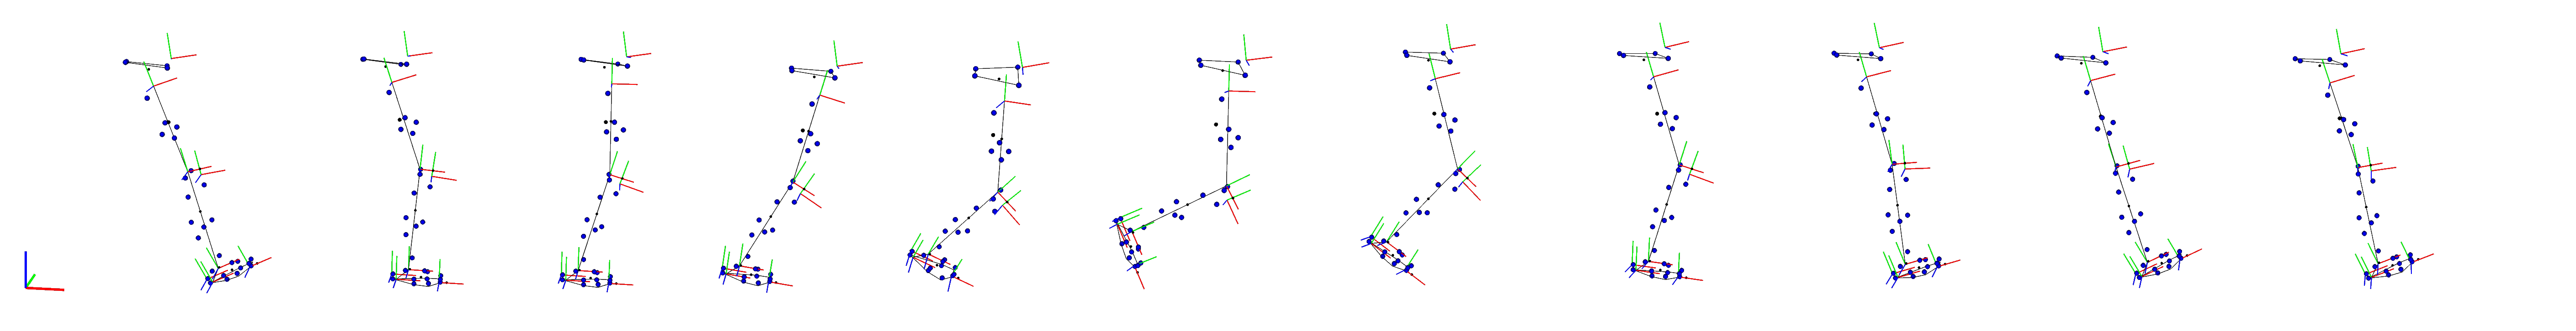
\includegraphics[width=\textwidth]{figures/multiphase_walking_cycle.png}\\
\caption{Snapshots of a walking gait cycle driven by torque actuators.}
\label{fig:snapshots_multiphase_walking_cycle}
\end{figure*}

%\begin{table}[h!]
%\caption{\small Objective terms of the Multiphase torque driven walking cycle }
%\label{tab:Multiphase_torque_driven_walking_cycle}
%\centering
%\begin{tabular}{c c c c}
%\toprule 
%& Type & Function & Weight \\ 
%\midrule
%$\#1$ & Lagrange & TRACK\_ STATE & $1e5$ \\ 
%\midrule
%$\#2$ & Lagrange & MINIMIZE\_ TORQUE\_ DERIVATIVE & $1e-2$ \\ 
%\midrule
%$\#3$ & Lagrange & TRACK\_ GRF & $1e-2$ \\ 
%\midrule
%$\#4$ & Lagrange & TRACK\_ MOMENTS & $1e-1$ \\
%\bottomrule
%\end{tabular}
%\end{table}
